\documentclass[11pt]{article}

% -------------------------------------------------
% Packages
% -------------------------------------------------
\usepackage[a4paper,margin=2.5cm]{geometry}
\usepackage{amsmath, amssymb, amsthm}
\usepackage{hyperref}
\usepackage{graphicx}
\usepackage{physics}
\usepackage{bm}

\hypersetup{
    colorlinks=true,
    linkcolor=blue,
    urlcolor=blue,
    citecolor=blue
}

% -------------------------------------------------
% Document Metadata
% -------------------------------------------------
\title{\textbf{The Ontology of Continua}\\
\vspace{0.3em}
\large A Unified Axiomatic Framework for Emergence, Persistence and Collapse}
\author{Alexander Yashin}
\date{v1.0-preprint}

% -------------------------------------------------
% Document
% -------------------------------------------------
\begin{document}

\maketitle
\tableofcontents
\newpage

% -------------------------------------------------
% Core Sections (existing in /tex)
% -------------------------------------------------

\section{Introduction}

Scientific models across physics, chemistry, biology and social systems rely on
domain-specific assumptions and formalisms. Despite their differences, these
domains exhibit structurally identical phenomena: the formation of stable
regimes, the emergence of new degrees of freedom, threshold-driven transitions,
and collapse under constraint violation. Current theories describe these
processes locally but lack a unified formal basis.

The Ontology of Continua (OC) introduces such a basis. A continuum is defined as
a structured system whose existence depends on the persistence of an admissible
state domain under dynamic constraints. A continuum is characterised by a compact
set of components:
\begin{itemize}
    \item axes of distinction $A$,
    \item potentials $P$,
    \item thresholds $\Theta$,
    \item fluxes $J$,
    \item cycles $C$,
    \item admissible domain $\Omega(K)$,
    \item boundary $\partial\Omega(K)$,
    \item structural tension $T$,
    \item continuity measure $k(t)$.
\end{itemize}

These components are combined by a universal operator
\[
\frac{dX_K}{dt} = (F,G,H,Q,R,S,U)(X_K,M),
\]
which governs the evolution of any continuum $K$ inside a metaspace $M$. The
operator formalises the conditions under which a continuum persists, expands its
dimensionality, or collapses.

OC provides a hierarchical structure $K_0$--$K_{12}$ describing how continua
emerge through successive increases in structural complexity. The hierarchy
spans proto-continua, physical fields, chemical reaction networks, protocells,
bioelectric systems, cognitive architectures, social institutions,
civilisational systems and formal-recursive metatheories. Each transition
$K_i \rightarrow K_{i+1}$ is defined by the appearance of a new axis of
distinction triggered when structural tension exceeds a critical threshold.

The objective of OC is to supply a unified axiomatic framework capable of
expressing emergence, stability, criticality and collapse across scientific
domains. This preprint presents the core axioms, the universal operator, the
K-level hierarchy, the formal continuity conditions, and the associated
falsifiability criteria.

\input{tex/axioms}
\input{tex/operator}
% hierarchy.tex
% Core v2.5 — Hierarchy of Continua K0–K12

\section{Hierarchy of Continua}
\label{sec:hierarchy}

This section provides the compact formal description of all continua
\(K_0,\dots,K_{12}\) as established in Core~v2.5.  
Each level is an instance of the universal template
\[
  K = (\Omega, A, P, \Theta, J, C, k).
\]
The hierarchy is generated by the conjugate chain
\[
  (K_0, M_1), (K_1, M_2), \dots, (K_{12}, M_{13}),
\]
where \(M_{x+1}\) is the metaspace induced by \(K_x\).

\subsection{Level \texorpdfstring{$K_0$}{K0}: Metalogical Layer}
\label{subsec:hierarchy-k0}

\begin{itemize}
  \item \textbf{Nature:} Not a physical layer; defines conditions of possibility.
  \item \textbf{State space:} Abstract metalogical domain.
  \item \textbf{Axes:} None; difference is meta-defined.
  \item \textbf{Potentials:} None.
  \item \textbf{Thresholds:} Logical consistency constraints.
  \item \textbf{Flows:} Metalogical inference.
  \item \textbf{Cycles:} Consistency-preserving loops in logic.
  \item \textbf{Continuumness:} \(k_0 = 1\) if \(\Omega(K_0)\neq\varnothing\), else \(0\).
\end{itemize}

\subsection{Level \texorpdfstring{$K_1$}{K1}: Lattice Continuum}
\label{subsec:hierarchy-k1}

\begin{itemize}
  \item \textbf{State space:} A discrete lattice \(X\).
  \item \textbf{Axes:} One axis \(A_1\) (occupancy or spin).
  \item \textbf{Potentials:} Local potentials \(P_1\).
  \item \textbf{Thresholds:} Connectivity threshold \(\Theta_1\).
  \item \textbf{Flows:} Neighbour interactions.
  \item \textbf{Cycles:} Minimal trivial cycle \(C_{\mathrm{triv}}\).
  \item \textbf{Continuumness:}  
    \[
      k_1(p) = \frac{|C_{\max}(p)|}{|X|}.
    \]
\end{itemize}

\subsection{Level \texorpdfstring{$K_2$}{K2}: Percolation Continuum}
\label{subsec:hierarchy-k2}

\begin{itemize}
  \item \textbf{State space:} Infinite lattice or continuum limit.
  \item \textbf{Axes:} Occupancy \(A_1\), cluster connectivity \(A_2\).
  \item \textbf{Potentials:} Bond probabilities.
  \item \textbf{Thresholds:} Percolation threshold \(\Theta_2 = p_c\).
  \item \textbf{Flows:} Cluster growth.
  \item \textbf{Cycles:} Trivial cycle with period \(\tau\propto\xi\).
  \item \textbf{Continuumness:}  
    \[
      k_2(p) = P_\infty(p).
    \]
\end{itemize}

\subsection{Level \texorpdfstring{$K_3$}{K3}: Autocatalytic Reaction Networks}
\label{subsec:hierarchy-k3}

\begin{itemize}
  \item \textbf{State space:} Concentrations and reaction graph.
  \item \textbf{Axes:} \(A_{\mathrm{chem}}\), \(A_{\mathrm{react}}\).
  \item \textbf{Potentials:} Chemical potentials and activities.
  \item \textbf{Thresholds:} Reaction feasibility \(\Theta_{\mathrm{react}}\).
  \item \textbf{Flows:} Reaction fluxes.
  \item \textbf{Cycles:} RAF-cycles.
  \item \textbf{Continuumness:}  
    \[
      k_3 \propto \frac{\text{RAF connectivity}}{\text{total network size}}.
    \]
\end{itemize}

\subsection{Level \texorpdfstring{$K_4$}{K4}: Protocellular Continuum}
\label{subsec:hierarchy-k4}

\begin{itemize}
  \item \textbf{State space:} Internal and external concentrations.
  \item \textbf{Axes:} Inside/outside axis, permeability axis, gradient axes.
  \item \textbf{Potentials:} Osmotic, electrochemical, metabolic.
  \item \textbf{Thresholds:} Membrane stability \(\Theta_{\mathrm{mem}}\).
  \item \textbf{Flows:} Transport through membrane, metabolic fluxes.
  \item \textbf{Cycles:} Metabolic cycles.
  \item \textbf{Continuumness:}  
    \[
      k_4 = f(\text{gradient stability},\ \text{cycle persistence}).
    \]
\end{itemize}

\subsection{Level \texorpdfstring{$K_5$}{K5}: Neuronal Continuum}
\label{subsec:hierarchy-k5}

\begin{itemize}
  \item \textbf{State space:} Membrane potentials and channel states.
  \item \textbf{Axes:} Excitability axis, channel axes, synaptic axes.
  \item \textbf{Potentials:} Electrical and chemical potentials.
  \item \textbf{Thresholds:} Excitation threshold \(\Theta_{\mathrm{spike}}\).
  \item \textbf{Flows:} Ion currents, neurotransmitter flows.
  \item \textbf{Cycles:} Spike cycles.
  \item \textbf{Continuumness:}  
    \[
      k_5 = H(\Omega)\cdot \frac{|V_{\mathrm{cycle}}|}{|V|} \cdot 
      \frac{\sum C^{\mathrm{eff}}}{\sum C^{\mathrm{max}}}.
    \]
\end{itemize}

\subsection{Level \texorpdfstring{$K_6$}{K6}: Cognitive Continuum}
\label{subsec:hierarchy-k6}

\begin{itemize}
  \item \textbf{State space:} Cognitive models and prediction states.
  \item \textbf{Axes:} Model axes \(A^{(6)}\), discrepancy axes.
  \item \textbf{Potentials:} Prediction error, valence, salience.
  \item \textbf{Thresholds:} Cognitive inconsistency \(\Theta_{\mathrm{cog}}\).
  \item \textbf{Flows:} Updates of models, information flows.
  \item \textbf{Cycles:} Model stability cycles.
  \item \textbf{Continuumness:}  
    \[
      k_6 = H(\Omega)\cdot
      \frac{|C_{\max}^{(6)}|}{|\mathcal{M}|}\cdot
      \frac{r}{r_{\max}}\cdot
      \left(1-\frac{D}{\Theta_{\mathrm{cog,max}}}\right)_+.
    \]
\end{itemize}

\subsection{Level \texorpdfstring{$K_7$}{K7}: Social Systems}
\label{subsec:hierarchy-k7}

\begin{itemize}
  \item \textbf{State space:} Agents, roles, norms.
  \item \textbf{Axes:} Social difference axes, role/norm axes.
  \item \textbf{Potentials:} Cooperation, trust, conflict potentials.
  \item \textbf{Thresholds:} Cooperation threshold \(\Theta_{\mathrm{coop}}\).
  \item \textbf{Flows:} Communication flows \(J_{\mathrm{comm}}\).
  \item \textbf{Cycles:} Institutional cycles \(C_{\mathrm{inst}}\).
  \item \textbf{Continuumness:}  
    \[
      k_7 = f(\text{communication coherence},\ \text{institutional cycles}).
    \]
\end{itemize}

\subsection{Level \texorpdfstring{$K_8$}{K8}: Civilizational Systems}
\label{subsec:hierarchy-k8}

\begin{itemize}
  \item \textbf{State space:} Institutions, infrastructures, symbolic systems.
  \item \textbf{Axes:} Technological, economic, legal, symbolic axes.
  \item \textbf{Potentials:} Stability, entropy, energy, innovation potentials.
  \item \textbf{Thresholds:} Stability threshold \(\Theta_{\mathrm{stab}}\).
  \item \textbf{Flows:} Resource flows, information flows, institutional flows.
  \item \textbf{Cycles:} Civilizational cycles \(C_{\mathrm{stab}}\).
  \item \textbf{Continuumness:}  
    \[
      k_8 = f(\text{infrastructure stability},\ \text{cycle persistence}).
    \]
\end{itemize}

\subsection{Level \texorpdfstring{$K_9$}{K9}: Metatheoretical Continuum}
\label{subsec:hierarchy-k9}

\begin{itemize}
  \item \textbf{State space:} Theories, paradigms, logics.
  \item \textbf{Axes:} Logical, ontological, methodological, interpretative axes.
  \item \textbf{Potentials:} Explanatory power, coherence, parsimony.
  \item \textbf{Thresholds:} Contradiction thresholds, empirical thresholds.
  \item \textbf{Flows:} Arguments, proofs, reinterpretations.
  \item \textbf{Cycles:} Scientific cycles.
  \item \textbf{Continuumness:}  
    \[
      k_9 = f(\text{coherence},\ \text{empirical adequacy}).
    \]
\end{itemize}

\subsection{Level \texorpdfstring{$K_{10}$}{K10}: Metamodel Continuum}
\label{subsec:hierarchy-k10}

\begin{itemize}
  \item \textbf{State space:} Categories of models.
  \item \textbf{Axes:} Functorial axes, structural axes.
  \item \textbf{Potentials:} Coherence and interpretability potentials.
  \item \textbf{Thresholds:} Coherence threshold.
  \item \textbf{Flows:} Functorial flows.
  \item \textbf{Cycles:} Functorial cycles.
  \item \textbf{Continuumness:}  
    \[
      k_{10} = f(\text{categorical coherence}).
    \]
\end{itemize}

\subsection{Level \texorpdfstring{$K_{11}$}{K11}: Meta-Semantic Continuum}
\label{subsec:hierarchy-k11}

\begin{itemize}
  \item \textbf{State space:} Semantic spaces of metamodels.
  \item \textbf{Axes:} Semantic, structural, interpretational axes.
  \item \textbf{Potentials:} Semantic coherence and expressivity.
  \item \textbf{Thresholds:} Semantic stability.
  \item \textbf{Flows:} Interpretation flows.
  \item \textbf{Cycles:} Meta-semantic cycles.
  \item \textbf{Continuumness:}  
    \[
      k_{11} = f(\text{semantic coherence}).
    \]
\end{itemize}

\subsection{Level \texorpdfstring{$K_{12}$}{K12}: Meta-Integrative Continuum}
\label{subsec:hierarchy-k12}

\begin{itemize}
  \item \textbf{State space:} Integration of all semantic/meta-theoretical levels.
  \item \textbf{Axes:} Integrative axes across metatheories.
  \item \textbf{Potentials:} Global coherence and integrability.
  \item \textbf{Thresholds:} Global integrability threshold.
  \item \textbf{Flows:} Cross-level integrative flows.
  \item \textbf{Cycles:} Global integrative cycles.
  \item \textbf{Continuumness:}  
    \[
      k_{12} = f(\text{global integrative consistency}).
    \]
\end{itemize}

% continuity.tex
% Core v2.5 — Continuity Conditions Across Levels

\section{Continuity Across Levels}
\label{sec:continuity}

This section formalises the continuity relations between successive levels
\(K_x \rightarrow K_{x+1}\) and the associated metaspaces \(M_{x+1}\).
Continuity ensures that the emergence of each higher-level continuum
respects the fundamental constraints imposed by its predecessor.

\subsection{Continuity Definition}
\label{subsec:continuity-definition}

Each level transition is governed by an operator
\[
  \Psi_{x \rightarrow x+1} : K_x \to K_{x+1},
\]
mapping states, axes, potentials, thresholds, flows, cycles, and
continuity data from one level to the next.

A transition is \emph{continuous} if and only if:

\begin{enumerate}
  \item \textbf{Admissibility preservation:}
    \[
      \Omega(K_x) \subseteq \Omega(M_{x+1}).
    \]

  \item \textbf{Axis extension:}
    \[
      A(K_x) \subseteq A(K_{x+1})
    \]
    and new axes appear only due to structural incompatibilities
    unresolvable within \(K_x\).

  \item \textbf{Threshold inheritance:}
    Thresholds of \(K_x\) remain valid constraints in \(K_{x+1}\);
    new thresholds \(\Theta_{x+1}\) appear only when required
    to stabilise new axes.

  \item \textbf{Cycle mapping:}
    Persistent cycles of \(K_x\) become sub-cycles of the cycles
    of \(K_{x+1}\):
    \[
      C(K_x) \subseteq C(K_{x+1}).
    \]

  \item \textbf{Continuity of \(k\):}
    \[
      k_x > 0 \implies k_{x+1} > 0.
    \]
\end{enumerate}

\subsection{Emergence of New Dimensions}
\label{subsec:continuity-dim}

Let \(\dim K_x\) denote the dimension of \(K_x\).
A dimension increase occurs when:

\begin{enumerate}
  \item A class of differences appears which cannot be represented on
    the existing axes of \(K_x\).

  \item Structural tension exceeds the dimensional threshold:
    \[
      T_x \ge \Theta^{\mathrm{dim}}_x.
    \]

  \item The metaspace \(M_{x+1}\) contains admissible configurations
    for the extended set of axes.
\end{enumerate}

Then:
\[
  \dim K_{x+1} = \dim K_x + 1.
\]

\subsection{Collapse Conditions}
\label{subsec:continuity-collapse}

A continuum \(K_x\) collapses if:

\begin{enumerate}
  \item All thresholds are violated:
    \[
      T(s) > \Theta(s) \quad \forall s \in S(K_x).
    \]

  \item No viable cycles remain:
    \[
      C(K_x) = \varnothing.
    \]

  \item The admissible region is empty:
    \[
      \Omega(K_x)=\varnothing.
    \]
\end{enumerate}

In this case,
\[
  k_x = 0.
\]

\subsection{Continuity Chain}
\label{subsec:continuity-chain}

The entire hierarchy satisfies the global continuity chain
\[
  K_0 \xrightarrow{\Psi_{0 \rightarrow 1}} K_1
     \xrightarrow{\Psi_{1 \rightarrow 2}} K_2
     \xrightarrow{\Psi_{2 \rightarrow 3}} K_3
     \xrightarrow{\Psi_{3 \rightarrow 4}} K_4
     \xrightarrow{\Psi_{4 \rightarrow 5}} K_5
     \xrightarrow{\Psi_{5 \rightarrow 6}} K_6
     \xrightarrow{\Psi_{6 \rightarrow 7}} K_7
     \xrightarrow{\Psi_{7 \rightarrow 8}} K_8
     \xrightarrow{\Psi_{8 \rightarrow 9}} K_9
     \xrightarrow{\Psi_{9 \rightarrow 10}} K_{10}
     \xrightarrow{\Psi_{10 \rightarrow 11}} K_{11}
     \xrightarrow{\Psi_{11 \rightarrow 12}} K_{12}.
\]

At each step,
\[
  k_x > 0 \ \Rightarrow\ k_{x+1} > 0,
\]
and dimensions grow monotonically unless collapse occurs.

\subsection{Minimal Conditions for Transition}
\label{subsec:continuity-minimal}

A transition \(K_x \to K_{x+1}\) is possible if and only if:

\begin{enumerate}
  \item \(\Omega(K_x) \neq \varnothing\).
  \item Structural tension satisfies:
    \[
      T_x \in [0, \Theta^{\mathrm{dim}}_x].
    \]
  \item A new axis \(A_{x+1}\) resolves incompatibilities in \(K_x\).
  \item \(M_{x+1}\) provides admissible states for the extended system.
\end{enumerate}

\subsection{Compact Summary}
\label{subsec:continuity-summary}

Continuity across levels is enforced by:

\begin{itemize}
  \item preservation of admissibility,
  \item faithful lifting of axes, potentials, and thresholds,
  \item persistence of cycles,
  \item compatibility with the metaspace,
  \item monotonic growth of dimension,
  \item non-zero continuity of the successor,
  \item and collapse only via loss of cycles and violation of all thresholds.
\end{itemize}

Together these conditions guarantee that the entire hierarchy
\(K_0 \to K_{12}\) forms a coherent unified structure.

\input{tex/transition-operators}
% falsifiability.tex
% Core v2.5 — Falsifiability and Empirical Tests

\section{Falsifiability and Empirical Tests}
\label{sec:falsifiability}

This section provides the universal and level-specific criteria under which
the Continuum Framework can be empirically or mathematically falsified.
Falsifiability is formulated directly in terms of the core components
\[
  (\Omega, A, P, \Theta, J, C, k).
\]

\subsection{Universal Falsifiability Criteria}
\label{subsec:falsifiability-universal}

The framework is falsifiable if any of the following universal conditions
are violated by observation, experiment, or mathematical proof.

\paragraph{Criterion F1 (Admissible Region Failure).}
There must exist non-empty admissible states:
\[
  \Omega(K) \neq \varnothing.
\]
If a continuum is claimed to exist but no admissible states exist under its
own constraints, the model is falsified.

\paragraph{Criterion F2 (Cycle Requirement).}
Continuumness is strictly tied to the existence of cycles:
\[
  k(K) > 0 \iff C(K) \neq \varnothing.
\]
If a living continuum is observed without any persistent cycle,
the theory is false.

\paragraph{Criterion F3 (Threshold Structure).}
Thresholds must separate admissible and inadmissible states:
\[
  T(s)\le0 \ \text{inside }\Omega,\qquad
  T(s)=0 \ \text{on }\partial\Omega.
\]
If thresholds do not regulate transitions as predicted, the model is falsified.

\paragraph{Criterion F4 (Monotonic Dimension).}
If a continuum remains alive (\(k>0\)) and its dimension decreases,
the theory is falsified.

\paragraph{Criterion F5 (Metaspace Compatibility).}
The existence condition
\[
  \Omega(K_x) \subseteq \Omega(M_x)
\]
must hold for every level.
Violation falsifies the framework.

\subsection{Level-Specific Tests}
\label{subsec:falsifiability-levels}

We summarise concrete falsification tests for each major level.

\paragraph{Physics (K1–K2).}
\begin{itemize}
  \item Violation of percolation threshold behaviour.
  \item Existence of connectivity without cycles in K1.
  \item Observation of time without any periodic process.
\end{itemize}

\paragraph{Chemistry (K3–K4).}
\begin{itemize}
  \item Autocatalytic networks persist with no cycles.
  \item Protocells maintain gradients without membrane thresholds.
  \item Transport occurs across membranes without crossing \(\Theta_{\mathrm{mem}}\).
\end{itemize}

\paragraph{Biology (K4–K6).}
\begin{itemize}
  \item Neurons spike without surpassing \(\Theta_{\mathrm{spike}}\).
  \item Cognitive systems stabilise models without cycles in their attractor space.
  \item Prediction-error dynamics violate the defined potentials.
\end{itemize}

\paragraph{Social Systems (K7).}
\begin{itemize}
  \item Stable institutions without communication cycles.
  \item Cooperation emerging below \(\Theta_{\mathrm{coop}}\).
  \item Social collapse occurring with all thresholds satisfied.
\end{itemize}

\paragraph{Civilizations (K8).}
\begin{itemize}
  \item Civilizational collapse without violation of \(\Theta_{\mathrm{stab}}\).
  \item Long-term stability without cycles \(C_{\mathrm{stab}}\).
\end{itemize}

\paragraph{Knowledge and Metatheory (K9–K12).}
\begin{itemize}
  \item Logical inconsistency in sustained paradigms (K9).
  \item Functorial incoherence in persistent metamodels (K10).
  \item Semantic instability despite all thresholds being satisfied (K11).
  \item Global integrative collapse without threshold violation (K12).
\end{itemize}

\subsection{Experimental and Observational Protocols}
\label{subsec:falsifiability-protocols}

The framework proposes domain-specific tests:

\paragraph{K2 Tests.}
Percolation experiments on lattices; measurement of \(P_\infty\).

\paragraph{K3 Tests.}
Sustained autocatalytic cycles under perturbation; reaction feasibility.

\paragraph{K4 Tests.}
Membrane osmotic collapse; transport thresholds; metabolic cycle persistence.

\paragraph{K5 Tests.}
Patch-clamp excitation threshold; spike cycle deformation; refractory thresholds.

\paragraph{K6 Tests.}
Cognitive inconsistency measurement; attractor stability; prediction-error thresholds.

\paragraph{K7 Tests.}
Institutional cycle duration; coherence of communication flows.

\paragraph{K8 Tests.}
Stability metrics of infrastructures; analysis of long-term civilizational cycles.

\paragraph{K9–K12 Tests.}
Logical coherence, structural mapping, semantic consistency.

\subsection{Meta-Falsifiability}
\label{subsec:falsifiability-meta}

The framework also predicts that:

\begin{itemize}
  \item Any model \(M\) representing a continuum must itself be a continuum
    under \(K_9\) or \(K_{10}\).
  \item Falsification of a model requires detecting violation of its own
    \((\Omega, A, P, \Theta, J, C, k)\).
  \item Meta-falsification occurs when an entire class of models violates
    metaspace constraints.
\end{itemize}

\subsection{Compact Summary}
\label{subsec:falsifiability-summary}

Falsifiability is encoded directly in the structure of continua:
\[
  K \text{ is false} \iff
  \bigl(
    \Omega=\varnothing \ \lor \
    C=\varnothing\text{ while }k>0 \ \lor \
    \dim\downarrow\text{ while }k>0 \ \lor \
    \Omega(K_x)\not\subseteq\Omega(M_x)
  \bigr).
\]
The framework is thus fully testable across all physical,
chemical, biological, cognitive, social, civilizational, and metatheoretical
domains.

% applications.tex
% Core v2.5 — Applications and Cross-Level Predictions

\section{Applications and Cross-Level Predictions}
\label{sec:applications}

The Continuum Framework provides a unified structural language that
connects physical, chemical, biological, cognitive, social and
civilisational systems.  
This section gives concrete examples of how the universal template
\[
  K = (\Omega, A, P, \Theta, J, C, k)
\]
can be used to analyse, compare, and predict the behaviour of real
systems across scientific domains.

Rather than focusing on phenomenological details, we highlight the
structural aspects of continua: admissibility, thresholds, cycles and
continuumness.  
These features appear in surprisingly similar ways across levels
\(K_0\)–\(K_{12}\).

\subsection{Percolation and Critical Connectivity (\texorpdfstring{$K_2$}{K2})}
\label{subsec:applications-k2}

In physics and network science, percolation is the canonical example
of a phase transition arising from local connectivity.  
In the continuum language:
\begin{itemize}
  \item The control parameter is the occupancy probability \(p\).
  \item The order parameter is the continuumness \(k_2(p)\), the
        probability that a randomly chosen node lies in the infinite
        cluster.
  \item The critical threshold is \(p_c\), where \(k_2\) becomes
        strictly positive.
\end{itemize}

\paragraph{Prediction 1: Universality of cycle emergence.}
Near the percolation threshold, the minimal cycle period \(\tau(K_2)\)
diverges as correlation length increases.  
Any system whose macroscopic behaviour depends on long-range
connectivity will exhibit the same increase in \(\tau\) as it
approaches the boundary \(\partial\Omega(K_2)\), even if the microscopic
physics is entirely different.

This provides a structural explanation of critical slowing down in:
\begin{itemize}
  \item magnetic systems near the Curie point,
  \item epidemic models near the epidemic threshold,
  \item information cascades in networks,
  \item congestion dynamics in traffic and communication systems.
\end{itemize}

\subsection{Protocellular Stability and Osmotic Limits (\texorpdfstring{$K_4$}{K4})}
\label{subsec:applications-k4}

A protocell is viable only if its membrane withstands osmotic, chemical
and mechanical stresses.  
In the continuum model:
\begin{itemize}
  \item osmotic gradients are potentials \(P_{\mathrm{grad}}\),
  \item membrane permeability is an axis \(A_{\mathrm{perm}}\),
  \item membrane rupture is defined by thresholds
        \(\Theta_{\mathrm{mem}}\),
  \item metabolic loops are cycles \(C_4\),
  \item protocellular integrity is measured by \(k_4(t)\).
\end{itemize}

\paragraph{Prediction 2: Linear instability of protocells near rupture.}
When osmotic pressure approaches the membrane threshold
\(\Theta_{\mathrm{mem}}\), structural tension grows linearly and the
time to rupture obeys:
\[
  \tau_{\mathrm{rupture}} \propto
  \frac{1}{\Theta_{\mathrm{mem}} - T_{\mathrm{mem}}}.
\]
This relationship predicts that protocells under slow environmental
changes exhibit a sudden collapse once tension surpasses the threshold,
mirroring percolation-like transitions.

\paragraph{Prediction 3: Minimal cycle condition for viability.}
A protocell with no stable metabolic cycle
\(C_4\neq\varnothing\) cannot maintain gradients and therefore cannot
keep \(k_4>0\).  
This yields a general viability constraint across all models of early
cellular life: at least one energy- or turnover-producing cycle must
remain operational for the system to remain inside \(\Omega(K_4)\).

\subsection{Neuronal Excitation and Spike Cycles (\texorpdfstring{$K_5$}{K5})}
\label{subsec:applications-k5}

In neuroscience, spike generation is a threshold phenomenon.  
The continuum model formalises:
\begin{itemize}
  \item membrane potential \(V(t)\) as a potential,
  \item channel states and synaptic weights as axes,
  \item spike threshold as \(\Theta_{\mathrm{spike}}\),
  \item ion currents as flows \(J_5\),
  \item spike cycles as \(C_{\mathrm{spike}}\),
  \item coherent network activity as \(k_5\).
\end{itemize}

\paragraph{Prediction 4: Universal spike onset condition.}
Across all biophysically realistic neurons:
\[
  T_{\mathrm{exc}} \ge \Theta_{\mathrm{spike}}
  \quad\Rightarrow\quad
  \text{spike onset as a phase transition.}
\]
Regardless of specific ion-channel models, spike initiation corresponds
to a structural crossing of the admissibility boundary
\(\partial\Omega(K_5)\).

\paragraph{Prediction 5: Stability requires cycle closure.}
Neurons or networks that fail to complete the spike cycle
(refractory return to baseline) leave \(\Omega(K_5)\).  
Thus, certain pathological states (e.g.\ depolarisation block,
epileptiform plateaus) are reinterpretations of \(k_5(t)\to 0\) due to
loss of cycle closure.

\subsection{Cognitive Collapse and Predictive Overload (\texorpdfstring{$K_6$}{K6})}
\label{subsec:applications-k6}

In cognitive systems:
\begin{itemize}
  \item internal models form axes \(A^{(6)}\),
  \item prediction error is a potential,
  \item cognitive thresholds \(\Theta_{\mathrm{PE}}\) determine when
        models must be revised,
  \item belief updates are flows \(J_6\),
  \item attractor cycles are \(C_6\),
  \item effective cognition corresponds to \(k_6>0\).
\end{itemize}

\paragraph{Prediction 6: Cognitive overload as threshold crossing.}
If prediction error exceeds \(\Theta_{\mathrm{PE}}\), internal models
collapse or are replaced.  
This formalises cognitive overload and disorganisation as a structural
phase transition:
\[
  D(m) > \Theta_{\mathrm{PE}}
  \quad\Rightarrow\quad
  k_6 \to 0.
\]

\paragraph{Prediction 7: Minimal-connectivity condition for coherent thought.}
The Framework predicts that cognitive continua require a largest
component of model interconnections of size:
\[
  \lvert C_{\max}^{(6)} \rvert
  \ge \alpha \lvert \mathcal{M} \rvert,
\]
where \(\alpha\) is a universal constant bounded between 0.2 and 0.4.
Below this value, cognition fragments into disconnected subsystems.

\subsection{Institutions and Social Collapse (\texorpdfstring{$K_7$}{K7})}
\label{subsec:applications-k7}

Social continua depend on communication coherence, shared norms and
institutional cycles.

\paragraph{Prediction 8: Collapse via cycle interruption.}
If an institutional cycle \(C_{\mathrm{inst}}\) loses one of its
necessary stages (formation, codification, enforcement, revision),
the system exits \(\Omega(K_7)\).  
Thus, institutional breakdown is equivalent to
\[
  C_{\mathrm{inst}} = \varnothing
  \quad\Rightarrow\quad
  k_7 = 0.
\]

\paragraph{Prediction 9: Social stress exhibits hysteresis.}
Due to the cycle-based nature of \(K_7\), reducing external stress does
not automatically restore pre-collapse dynamics.  
The Framework predicts a hysteresis loop in the recovery of \(k_7\),
analogous to civilisational hysteresis in \(K_8\).

\subsection{Civilisational Stability and Long Waves (\texorpdfstring{$K_8$}{K8})}
\label{subsec:applications-k8}

Civilisations maintain a non-zero \(k_8\) by sustaining cycles such as:
\begin{itemize}
  \item food and energy production,
  \item infrastructure maintenance,
  \item administrative and legal reproduction,
  \item symbolic and cultural continuity.
\end{itemize}

\paragraph{Prediction 10: Collapse when civilisational tension exceeds thresholds.}
Let \(T_8\) be the civilisational tension—a composite measure of
resource stress, institutional overload and infrastructural fragility.
The Framework predicts:
\[
  T_8 > \Theta_{\mathrm{stab}}
  \quad\Rightarrow\quad
  \text{systemic collapse or reorganisation.}
\]

\paragraph{Prediction 11: Long-wave oscillations from cycle interaction.}
Interference of multiple stabilising cycles \(C_8\) produces long-wave
dynamics (50–200 year cycles) that appear in historical data.  
These oscillations are structurally equivalent to neural rhythms in
\(K_5\) or metabolic cycles in \(K_4\).

\subsection{Metatheoretical and Semantic Stability (\texorpdfstring{$K_9$--$K_{11}$}{K9--K11})}
\label{subsec:applications-k9-k11}

The Framework predicts cross-level analogies between theoretical,
semantic and physical stability.

\paragraph{Prediction 12: Paradigm stability requires cycle closure.}
Scientific paradigms correspond to cycles of theory creation,
prediction, testing and correction.  
If this cycle breaks, \(\Omega(K_9)\) collapses and the paradigm must
transition to a new one.

\paragraph{Prediction 13: Semantic drift as threshold process.}
Meaning systems lose coherence when ambiguity exceeds semantic
thresholds \(\Theta_{\mathrm{sem}}\).  
Thus semantic drift is the analogue of cognitive collapse or membrane
rupture.

\subsection{Artificial Systems and Integration (\texorpdfstring{$K_{12}$}{K12})}
\label{subsec:applications-k12}

In artificial systems, continua appear in:
\begin{itemize}
  \item distributed AI systems,
  \item multi-agent reinforcement learning,
  \item large-scale computational infrastructures.
\end{itemize}

\paragraph{Prediction 14: Integration requires cross-level coherence.}
Artificial systems embedded in human environments must satisfy:
\[
  \Omega(K_{\mathrm{artificial}}) \subseteq \Omega(K_{12})
\]
for stable integration.  
Violations correspond to misalignment, instability or unintended
behaviour.

\paragraph{Prediction 15: Artificial collapse mirrors natural collapse.}
If agent interactions fail to maintain internal cycles (coordination,
consensus, update, correction), artificial systems undergo collapse
structurally identical to that of institutions or civilisations.

\subsection{Summary of Cross-Level Analogies}
\label{subsec:applications-summary}

Despite differences in content and scale, many systems share:
\begin{itemize}
  \item threshold-induced phase transitions,
  \item cycle-based temporal structure,
  \item an order parameter measuring coherence (continuumness),
  \item admissible-state boundaries and collapse conditions.
\end{itemize}

These analogies make it possible to import results from one domain
(percolation, membrane physics, neuronal spiking, social systems,
civilisational models) into others in a controlled and formally
well-defined way.  
The Continuum Framework therefore serves not only as a theoretical
unification, but also as a generator of cross-domain predictions.

% bibliography_structure.tex
% Core v2.5 — Bibliography Structure

\section*{Bibliography}
\addcontentsline{toc}{section}{Bibliography}

% --------------------------------------------------------------------
% If you use BibTeX (recommended for the Continuum Project):
% --------------------------------------------------------------------

% Uncomment the following line once references.bib exists
% \bibliographystyle{plain}
% \bibliography{references}

% --------------------------------------------------------------------
% If you prefer manual entries (not recommended for long documents):
% --------------------------------------------------------------------

\begin{thebibliography}{99}

% --------------------------------------------------
% Physics (K0–K2)
% --------------------------------------------------
\bibitem{percolation}
D.~Stauffer and A.~Aharony.
\newblock {\em Introduction to Percolation Theory}.
\newblock Taylor and Francis, 1991.

\bibitem{bkt}
V.~L.~Berezinskii.
\newblock Destruction of Long-range Order in One-dimensional and
Two-dimensional Systems.
\newblock {\em Sov. Phys. JETP}, 32:493--500, 1971.

\bibitem{kosterlitz}
J.~M.~Kosterlitz and D.~J.~Thouless.
\newblock Ordering, metastability and phase transitions in two-dimensional
systems.
\newblock {\em J. Phys. C}, 6:1181--1203, 1973.

% --------------------------------------------------
% Chemistry (K3–K4)
% --------------------------------------------------
\bibitem{raf-eigen}
S.~A.~Kauffman.
\newblock Autocatalytic sets of proteins.
\newblock {\em J. Theor. Biol.}, 119:1--24, 1986.

\bibitem{szostak}
J.~W.~Szostak.
\newblock Protocells and the origin of cellular life.
\newblock {\em Annu. Rev. Biochem.}, 81:335--360, 2012.

% --------------------------------------------------
% Biology (K4–K5)
% --------------------------------------------------
\bibitem{hodgkin-huxley}
A.~L.~Hodgkin and A.~F.~Huxley.
\newblock A quantitative description of membrane current and its application
to conduction and excitation in nerve.
\newblock {\em J. Physiol.}, 117:500--544, 1952.

\bibitem{spike-initiation}
E.~M.~Izhikevich.
\newblock Simple model of spiking neurons.
\newblock {\em IEEE Trans. Neural Networks}, 14:1569--1572, 2003.

% --------------------------------------------------
% Cognition (K6)
% --------------------------------------------------
\bibitem{predictive-processing}
K.~Friston.
\newblock The free-energy principle: a unified brain theory?
\newblock {\em Nat. Rev. Neurosci.}, 11:127--138, 2010.

% --------------------------------------------------
% Social Systems (K7)
% --------------------------------------------------
\bibitem{luhmann}
N.~Luhmann.
\newblock {\em Social Systems}.
\newblock Stanford University Press, 1995.

% --------------------------------------------------
% Civilisation (K8)
% --------------------------------------------------
\bibitem{turchin}
P.~Turchin.
\newblock {\em Cliodynamics: The Journal of Quantitative History and Cultural
Evolution}, various articles.

% --------------------------------------------------
% Metatheory (K9–K11)
% --------------------------------------------------
\bibitem{kun}
T.~S.~Kuhn.
\newblock {\em The Structure of Scientific Revolutions}.
\newblock University of Chicago Press, 1962.

% --------------------------------------------------
% Artificial Systems (K12)
% --------------------------------------------------
\bibitem{distributed-ai}
B.~Grosz and S.~Kraus.
\newblock Collaborative multi-agent planning.
\newblock {\em AI Magazine}, 20:39--52, 1999.

\end{thebibliography}


% -------------------------------------------------
% Appendices (already in your repo)
% -------------------------------------------------

\appendix
% appendix_core.tex
% Core v2.5 — Appendix A: Core Mathematical Definitions

\section{Appendix A: Core Mathematical Definitions}
\label{sec:appendix-core}

This appendix provides the formal mathematical definitions underlying the
Continuum Framework. It expands the compact core specification
\[
  K = (\Omega, A, P, \Theta, J, C, k)
\]
into explicit structures suitable for mathematical analysis.

\subsection{State Space}
\label{subsec:appendix-core-state}

Each continuum \(K\) possesses a state space
\[
  S(K),
\]
which may be discrete, continuous, mixed, or categorical.
The admissible region is a subset \(\Omega(K)\subseteq S(K)\).

\subsection{Axes of Difference}
\label{subsec:appendix-core-axes}

Axes are measurable or distinguishable coordinates:
\[
  A_j : S(K) \to \mathcal{A}_{A_j}.
\]
The set of all axes is:
\[
  A(K) = \{ A_j \}_{j \in J_A}.
\]

\subsection{Potentials}
\label{subsec:appendix-core-potentials}

Potentials quantify forces or constraints:
\[
  P_i : S(K) \to \mathcal{D}_{P_i}.
\]

\subsection{Thresholds}
\label{subsec:appendix-core-thresholds}

Thresholds define admissibility boundaries:
\[
  \Theta_\ell : S(K) \to \mathbb{R}.
\]
All thresholds form a vector:
\[
  \vec{\Theta} = (\Theta_\ell)_{\ell\in J_\Theta}.
\]

\subsection{Flows}
\label{subsec:appendix-core-flows}

Flows describe transport or influence:
\[
  J_m : S(K)\times\mathbb{R} \to \mathcal{F}_m.
\]
Set of flows:
\[
  J(K) = \{J_m\}_{m\in J_J}.
\]

\subsection{Cycles}
\label{subsec:appendix-core-cycles}

Cycles are closed trajectories:
\[
  C_n : [0,\tau_n] \to S(K),
  \qquad C_n(0)=C_n(\tau_n).
\]

\subsection{Continuumness}
\label{subsec:appendix-core-k}

Continuumness is:
\[
  k : \Omega(K)\to[0,1].
\]

\subsection{Structural Tension}
\label{subsec:appendix-core-tension}

Structural tension is a scalar or vector field:
\[
  T : S(K)\to\mathbb{R},
\]
with sign indicating whether thresholds are satisfied:
\[
  T(s)\le0 \Rightarrow s\in\Omega(K), \qquad
  T(s)=0 \Rightarrow s\in\partial\Omega(K).
\]

\subsection{Boundary of Admissibility}
\label{subsec:appendix-core-boundary}

\[
  \partial\Omega(K) =
  \bigl\{ s \in S(K) \ \big|\ 
    T(s)=0 \lor 
    P_i(s)\in\partial\mathcal{D}_{P_i} \lor
    A_j(s)\in\partial\mathcal{A}_{A_j}
  \bigr\}.
\]

\subsection{Evolution Operator}
\label{subsec:appendix-core-evolution}

Dynamics are governed by:
\[
  E : K(t)\mapsto K(t+\Delta t),
\]
with component-wise updates:
\begin{align*}
  \frac{dA}{dt} &= F(A,P,\Theta,J,C,t), \\
  \frac{dP}{dt} &= G(A,P,\Theta,J,C,t), \\
  \frac{d\Theta}{dt} &= H(A,P,\Theta,J,C,t), \\
  \frac{dJ}{dt} &= Q(A,P,\Theta,J,C,t), \\
  \frac{dC}{dt} &= S(A,P,\Theta,J,C,t), \\
  \frac{dk}{dt} &= U(A,P,\Theta,J,C,k,t).
\end{align*}

\subsection{Time Scale}
\label{subsec:appendix-core-time}

If cycles exist:
\[
  \tau(K)=\min_n \tau_n.
\]
Otherwise:
\[
  \tau(K)=+\infty, \qquad k=0.
\]

\subsection{Dimension}
\label{subsec:appendix-core-dimension}

Dimension is defined via the number of independent axes:
\[
  \dim K = |A(K)|.
\]

\subsection{Dimension Growth}
\label{subsec:appendix-core-dim-growth}

A new dimension emerges when:
\[
  T\ge \Theta_{\mathrm{dim}}
  \quad\text{and}\quad
  \Omega(K_x)\subseteq\Omega(M_{x+1}).
\]

\subsection{Collapse Conditions}
\label{subsec:appendix-core-collapse}

Collapse occurs if:
\[
  \Omega=\varnothing
  \quad\text{or}\quad
  C=\varnothing.
\]

\subsection{Compatibility with Metaspace}
\label{subsec:appendix-core-compatibility}

For existence:
\[
  \Omega(K_x)\subseteq\Omega(M_x).
\]

\subsection{Compact Summary}
\label{subsec:appendix-core-summary}

This appendix formalises all core components:
\[
  S,\Omega,A,P,\Theta,J,C,k,T,\partial\Omega,E,\tau,\dim.
\]
These definitions provide the mathematical foundation of every level
\(K_0\) through \(K_{12}\).

% appendix_continuity.tex
% Core v2.5 — Appendix B: Continuity and Transition Operators

\section{Appendix B: Continuity and Transition Operators}
\label{sec:appendix-continuity}

This appendix provides the detailed mathematical formalisation of continuity
conditions, dimensional transitions, and collapse criteria used to define
inter-level dynamics in the Continuum Framework.

\subsection{Transition Operators}
\label{subsec:appendix-continuity-psi}

Each transition \(K_x \to K_{x+1}\) is generated by a transition operator
\[
  \Psi_{x\rightarrow x+1} : K_x \longrightarrow K_{x+1}
\]
acting on all components:
\[
  \Psi_{x\rightarrow x+1}(\Omega, A, P, \Theta, J, C, k)
  =
  (\Omega', A', P', \Theta', J', C', k').
\]

\subsection{Continuity Conditions}
\label{subsec:appendix-continuity-cond}

A transition is \emph{continuous} if the following hold:

\paragraph{(C1) Admissibility Preservation.}
\[
  \Omega(K_x) \subseteq \Omega(M_{x+1}).
\]

\paragraph{(C2) Axis Extension.}
\[
  A(K_x) \subseteq A(K_{x+1}), \qquad
  A(K_{x+1}) = A(K_x)\cup\{A_{\mathrm{new}}\}.
\]

\paragraph{(C3) Threshold Inheritance.}
\[
  \Theta(K_x)\subseteq\Theta(K_{x+1})
\]
and new thresholds correspond only to new axes.

\paragraph{(C4) Cycle Embedding.}
Every cycle in \(K_x\) persists as a sub-cycle in \(K_{x+1}\).

\paragraph{(C5) Continuity Preservation.}
\[
  k_x>0 \implies k_{x+1}>0.
\]

\subsection{Dimension Emergence}
\label{subsec:appendix-continuity-dim}

A new axis appears only when the following criteria are satisfied:

\paragraph{(D1) Structural Incompatibility.}
Existing axes cannot represent a new class of differences.

\paragraph{(D2) Dimensional Tension.}
\[
  T_x \ge \Theta_x^{\mathrm{dim}}.
\]

\paragraph{(D3) Metaspace Admissibility.}
\[
  \Omega(K_x) \subseteq \Omega(M_{x+1})
  \quad\text{and}\quad
  \Omega(K_{x+1}) \subseteq \Omega(M_{x+1}).
\]

If so:
\[
  \dim K_{x+1} = \dim K_x + 1.
\]

\subsection{Collapse Conditions}
\label{subsec:appendix-continuity-collapse}

Collapse occurs if any of the following hold:

\paragraph{(CL1) Loss of Admissibility.}
\[
  \Omega = \varnothing.
\]

\paragraph{(CL2) Loss of Cycles.}
\[
  C = \varnothing.
\]

\paragraph{(CL3) Threshold Violation.}
\[
  T(s) > \Theta(s) \ \forall s\in S(K).
\]

\paragraph{(CL4) Metaspace Violation.}
\[
  \Omega(K) \not\subseteq \Omega(M).
\]

In collapse:
\[
  k = 0.
\]

\subsection{Time Continuity}
\label{subsec:appendix-continuity-time}

Let the cycle periods of \(K_x\) be \(\{\tau_n^x\}\).
Then time is continuous across levels if:
\[
  \tau(K_{x+1}) \le \tau(K_x) \quad\text{or}\quad
  \tau(K_{x+1}) = \tau(K_x).
\]
If cycles expand without bound:
\[
  \tau(K_x)\to +\infty,
\]
the continuum is dead.

\subsection{Path Continuity in State Space}
\label{subsec:appendix-continuity-path}

A trajectory \(s(t)\) is continuous across levels if:
\[
  s(t)\in\Omega(K_x)
  \quad\text{and}\quad
  \Psi_{x\rightarrow x+1}(s(t))\in\Omega(K_{x+1})
\]
for all relevant \(t\).

\subsection{Metaspace Chain Conditions}
\label{subsec:appendix-continuity-meta}

The metaspace chain obeys:

\[
  \Omega(K_x)\subseteq\Omega(M_x), \qquad
  A(K_x)\subseteq A(M_x).
\]

Furthermore:
\[
  \mathrm{DoF}(K_x)\le \mathrm{DoF}(M_{x+1}).
\]

\subsection{Compact Summary}
\label{subsec:appendix-continuity-summary}

Transition operators formalise the hierarchy:

\[
  K_0 \xrightarrow{\Psi_{0\rightarrow1}} K_1
     \xrightarrow{\Psi_{1\rightarrow2}} K_2
     \dots
     \xrightarrow{\Psi_{11\rightarrow12}} K_{12}.
\]

Continuity requires:
\[
  \Omega_x\subseteq\Omega_{M_{x+1}},\ 
  A_x\subseteq A_{x+1},\ 
  C_x\subseteq C_{x+1},\ 
  k_x>0\Rightarrow k_{x+1}>0.
\]

Dimension grows monotonically, and collapse occurs only through loss of cycles
or violation of all thresholds.

% appendix_params.tex
% Core v2.5 — Appendix C: Parameters, Thresholds, and Tension Functions

\section{Appendix C: Parameters, Thresholds, and Tension Functions}
\label{sec:appendix-params}

This appendix defines the parameter sets, threshold functions, and tension
structures used across levels \(K_0\) to \(K_{12}\).  
Parameters include numerical values, functional dependencies, and structural
coefficients that shape the admissible region \(\Omega(K)\) and its boundary
\(\partial\Omega(K)\).

\subsection{Parameter Sets}
\label{subsec:appendix-params-sets}

For each continuum \(K\), the parameter set is:
\[
  \Pi(K) = \{\, \pi_1, \pi_2, \dots, \pi_n \,\},
\]
with each parameter \(\pi_i\) belonging to an admissible domain
\(\mathcal{D}_{\pi_i}\).

Examples include:
\begin{itemize}
  \item physical parameters (bond probability \(p\), coupling strengths),
  \item chemical parameters (rate constants, activities),
  \item biological parameters (channel densities, conductances),
  \item cognitive parameters (prediction-error bounds),
  \item social parameters (communication rates),
  \item civilizational parameters (resource throughput),
  \item metatheoretical parameters (coherence coefficients).
\end{itemize}

\subsection{Threshold Functions}
\label{subsec:appendix-params-thresholds}

Thresholds regulate transitions and define the admissible surface:
\[
  \Theta : S(K) \to \mathbb{R}.
\]

Each threshold may depend on parameters:
\[
  \Theta(s) = \Theta(s;\Pi).
\]

Key threshold classes include:
\begin{itemize}
  \item \emph{dimensional thresholds} \(\Theta_{\mathrm{dim}}\),
  \item \emph{stability thresholds} \(\Theta_{\mathrm{stab}}\),
  \item \emph{reactivity thresholds} \(\Theta_{\mathrm{react}}\),
  \item \emph{membrane thresholds} \(\Theta_{\mathrm{mem}}\),
  \item \emph{excitation thresholds} \(\Theta_{\mathrm{spike}}\),
  \item \emph{cognitive thresholds} \(\Theta_{\mathrm{cog}}\),
  \item \emph{cooperation thresholds} \(\Theta_{\mathrm{coop}}\),
  \item \emph{semantic thresholds} \(\Theta_{\mathrm{sem}}\).
\end{itemize}

\subsection{Threshold Surfaces}
\label{subsec:appendix-params-surfaces}

The admissible boundary is defined by:
\[
  T(s) = \Theta(s;\Pi)
  \qquad \iff \qquad
  s\in \partial\Omega(K).
\]

The structure may be:
\begin{itemize}
  \item smooth,
  \item nonlinear,
  \item piecewise-defined,
  \item discontinuous.
\end{itemize}

\subsection{Tension Function}
\label{subsec:appendix-params-tension}

Structural tension is defined as:
\[
  T : S(K)\to\mathbb{R},
\]
with the semantics:
\[
  T<0 \Rightarrow s\in \Omega(K), \qquad
  T=0 \Rightarrow s\in \partial\Omega(K), \qquad
  T>0 \Rightarrow s\notin\Omega(K).
\]

Tension may depend on potentials and flows:
\[
  T = f(P, J, \Pi).
\]

\subsection{Composite Thresholds}
\label{subsec:appendix-params-composite}

Some transitions require multiple thresholds simultaneously:
\[
  T_1 \le \Theta_1,\quad
  T_2 \le \Theta_2,\quad
  \dots,\quad
  T_m \le \Theta_m.
\]

The admissible region then satisfies:
\[
  \Omega(K)=\{s:\max_k (T_k(s)-\Theta_k(s))\le0\}.
\]

\subsection{Parameter Evolution}
\label{subsec:appendix-params-evolution}

Parameters may evolve:
\[
  \frac{d\Pi}{dt} = W(A,P,\Theta,J,C,k,\Pi,t)
\]
where \(W\) is an operator describing:

\begin{itemize}
  \item adaptation,
  \item learning,
  \item evolution,
  \item institutional change,
  \item semantic drift.
\end{itemize}

\subsection{Landscape Interpretation}
\label{subsec:appendix-params-landscape}

Thresholds and tension define a landscape:
\[
  L(s) = T(s) - \Theta(s;\Pi).
\]
The sign determines position relative to \(\Omega\).

Phase transitions occur when the landscape touches zero.

\subsection{Examples by Level}
\label{subsec:appendix-params-levels}

\paragraph{K2 (Percolation).}
\[
  \Theta_{\mathrm{dim}} = p_c,\quad
  T = p - p_c.
\]

\paragraph{K3 (Autocatalytic Chemistry).}
\[
  \Theta_{\mathrm{react}}=0, \quad
  T = \Delta G.
\]

\paragraph{K4 (Protocells).}
\[
  T = \Pi_{\mathrm{osm}} - \Pi_{\mathrm{mem}},
\]
with \(\Pi_{\mathrm{mem}}\) determined by membrane parameters.

\paragraph{K5 (Neurons).}
\[
  \Theta_{\mathrm{spike}} = V_{\mathrm{thr}},
  \qquad T = V - V_{\mathrm{thr}}.
\]

\paragraph{K6 (Cognition).}
\[
  \Theta_{\mathrm{cog}} = \Theta_{\mathrm{PE}}, \quad
  T = D(m) - \Theta_{\mathrm{PE}}.
\]

\paragraph{K7 (Social Systems).}
\[
  T = T_{\mathrm{comm}} - \Theta_{\mathrm{coop}}.
\]

\paragraph{K8 (Civilizations).}
\[
  T = T_{\mathrm{inst}} - \Theta_{\mathrm{stab}}.
\]

\paragraph{K9–K12 (Metatheory).}
\[
  T = \text{logical or semantic inconsistency measure}.
\]

\subsection{Compact Summary}
\label{subsec:appendix-params-summary}

This appendix defines all parameter sets, tension functions, and thresholds
across levels. These determine:

\begin{itemize}
  \item the shape of \(\Omega(K)\),
  \item the location of \(\partial\Omega(K)\),
  \item all phase transitions,
  \item the emergence of new axes,
  \item and collapse conditions.
\end{itemize}

The formalism is universal across physics, chemistry, biology, cognition,
social systems, civilizations, and metatheoretical levels.

% appendix_notation.tex
% Core v2.5 — Appendix D: Notation and Symbol Glossary

\section{Appendix D: Notation and Symbol Glossary}
\label{sec:appendix-notation}

This appendix defines all symbols, functions, operators, and sets used in the
Continuum Framework.  
It serves as a reference for the mathematical notation used throughout all
chapters and appendices.

\subsection{Sets and Spaces}
\label{subsec:appendix-notation-sets}

\begin{itemize}
  \item \(S(K)\) — state space of continuum \(K\).
  \item \(\Omega(K)\subseteq S(K)\) — admissible states.
  \item \(\partial\Omega(K)\subseteq S(K)\) — boundary of admissibility.
  \item \(M_x\) — metaspace associated with \(K_x\).
  \item \(\mathcal{A}_{A_j}\) — domain of axis \(A_j\).
  \item \(\mathcal{D}_{P_i}\) — domain of potential \(P_i\).
  \item \(\mathcal{D}_{\pi_i}\) — domain of parameter \(\pi_i\).
  \item \(J_A,J_P,J_\Theta,J_J,J_C\) — index sets for components.
\end{itemize}

\subsection{Core Components}
\label{subsec:appendix-notation-core}

\begin{itemize}
  \item \(A(K)=\{A_j\}\) — axes of difference.
  \item \(P(K)=\{P_i\}\) — potentials.
  \item \(\Theta(K)=\{\Theta_\ell\}\) — thresholds.
  \item \(J(K)=\{J_m\}\) — flows.
  \item \(C(K)=\{C_n\}\) — cycles.
  \item \(k(K):\Omega(K)\to[0,1]\) — continuumness.
  \item \(T(s)\) — structural tension in state \(s\).
\end{itemize}

\subsection{Operators}
\label{subsec:appendix-notation-operators}

\begin{itemize}
  \item \(E\) — evolution operator.
  \item \(\Psi_{x\rightarrow x+1}\) — transition operator.
  \item \(F,G,H,Q,S,U\) — component evolution operators for the dynamics.
  \item \(W\) — parameter evolution operator.
\end{itemize}

\subsection{Dynamics}
\label{subsec:appendix-notation-dynamics}

Differential relations:
\begin{align*}
  \frac{dA}{dt} &= F(A,P,\Theta,J,C,t), \\
  \frac{dP}{dt} &= G(A,P,\Theta,J,C,t), \\
  \frac{d\Theta}{dt} &= H(A,P,\Theta,J,C,t), \\
  \frac{dJ}{dt} &= Q(A,P,\Theta,J,C,t), \\
  \frac{dC}{dt} &= S(A,P,\Theta,J,C,t), \\
  \frac{dk}{dt} &= U(A,P,\Theta,J,C,k,t), \\
  \frac{d\Pi}{dt} &= W(A,P,\Theta,J,C,k,\Pi,t).
\end{align*}

\subsection{Temporal Quantities}
\label{subsec:appendix-notation-time}

\begin{itemize}
  \item \(\tau_n\) — period of cycle \(C_n\).
  \item \(\tau(K)\) — minimal cycle period:
  \[
    \tau(K)=\min_n \tau_n.
  \]
\end{itemize}

\subsection{Dimensions}
\label{subsec:appendix-notation-dim}

\begin{itemize}
  \item \(\dim K = |A(K)|\) — number of axes.
  \item \(\Theta_{\mathrm{dim}}\) — dimensional threshold.
  \item \(\mathrm{DoF}(K)\) — degrees of freedom of \(K\).
\end{itemize}

\subsection{Threshold Structures}
\label{subsec:appendix-notation-thresholds}

\begin{itemize}
  \item Stability thresholds \(\Theta_{\mathrm{stab}}\).
  \item Reaction thresholds \(\Theta_{\mathrm{react}}\).
  \item Membrane thresholds \(\Theta_{\mathrm{mem}}\).
  \item Spike thresholds \(\Theta_{\mathrm{spike}}\).
  \item Cognitive thresholds \(\Theta_{\mathrm{cog}}\).
  \item Cooperation thresholds \(\Theta_{\mathrm{coop}}\).
  \item Semantic thresholds \(\Theta_{\mathrm{sem}}\).
\end{itemize}

\subsection{Tension}
\label{subsec:appendix-notation-tension}

\[
  T : S(K)\to\mathbb{R}
\]
indicates structural tension.

\subsection{Parameter Sets}
\label{subsec:appendix-notation-params}

\[
  \Pi(K) = \{\pi_1,\dots,\pi_n\}.
\]

\subsection{Metaspace Conditions}
\label{subsec:appendix-notation-meta}

\[
  \Omega(K_x)\subseteq\Omega(M_x), \qquad
  A(K_x)\subseteq A(M_x).
\]
\[
  \mathrm{DoF}(K_x)\le\mathrm{DoF}(M_{x+1}).
\]

\subsection{Glossary of Frequently Used Symbols}
\label{subsec:appendix-notation-glossary}

\begin{itemize}
  \item \(s\) — state of the continuum.
  \item \(\partial\Omega\) — boundary of admissibility.
  \item \(L(s)=T(s)-\Theta(s)\) — landscape function.
  \item \(p_c\) — percolation threshold.
  \item \(V_{\mathrm{thr}}\) — voltage threshold.
  \item \(D(m)\) — cognitive discrepancy.
  \item \(T_{\mathrm{comm}}\) — communication tension.
  \item \(T_{\mathrm{inst}}\) — institutional tension.
\end{itemize}

\subsection{Compact Summary}
\label{subsec:appendix-notation-summary}

This appendix provides a complete glossary of symbols across all levels
\(K_0\) to \(K_{12}\).  
It ensures consistency of notation and enables cross-level analysis using a
single unified symbolic system.

% appendix_levels.tex
% Core v2.5 — Appendix E: Level Definitions K0–K12

\section{Appendix E: Level Definitions \texorpdfstring{$K_0$--$K_{12}$}{K0--K12}}
\label{sec:appendix-levels}

This appendix provides compact but fully formal definitions of all continua
\(
  K_0, K_1, \dots, K_{12}
\),
each as an instance of the universal structure
\[
  K = (\Omega, A, P, \Theta, J, C, k).
\]

We write \(\Omega_x=\Omega(K_x)\), \(A_x=A(K_x)\),  
\(P_x=P(K_x)\), \(\Theta_x=\Theta(K_x)\),  
\(J_x=J(K_x)\), \(C_x=C(K_x)\), and \(k_x=k(K_x)\).

Each level satisfies:

\[
  \Omega_x\neq\varnothing \;\wedge\; C_x\neq\varnothing
  \;\Longleftrightarrow\; k_x>0,
\]
and
\[
  k_x>0\Rightarrow \dim K_{x+1} \ge \dim K_x.
\]

% ============================================================
\subsection{\texorpdfstring{$K_0$}{K0}: Meta-Logical Continuum}
\label{subsec:appendix-levels-k0}

\paragraph{State space.}
\[
  S(K_0)=\mathcal{P}\times\mathcal{L},
\]
conditions of possibility \(\mathcal{P}\) and metalaws \(\mathcal{L}\).

\paragraph{Axes.}
No internal axes:
\[
  A_0=\varnothing.
\]

\paragraph{Potentials and thresholds.}
Potentials encode consistency; thresholds are logical constraints.

\paragraph{Flows and cycles.}
Inference flows; consistency cycles.  
Continuumness:
\[
  k_0 =
  \begin{cases}
    1,& \Omega_0\neq\varnothing,\\
    0,& \text{otherwise}.
  \end{cases}
\]

% ============================================================
\subsection{\texorpdfstring{$K_1$}{K1}: One-Dimensional Continuum}
\label{subsec:appendix-levels-k1}

\paragraph{State space.}
\[
  S(K_1)=\{\,s:X\to V\,\},
\]
local states on a finite lattice \(X\).

\paragraph{Axes.}
Single axis \(A_1\) (local state: occupied/vacant or spin).

\paragraph{Potentials.}
Local energies, couplings.

\paragraph{Thresholds.}
Connectivity/percolation-like threshold \(\Theta_1\).

\paragraph{Flows and cycles.}
Neighbour flows, trivial closure cycle.  
\[
  k_1(p)=\frac{|C_{\max}(p)|}{|X|}.
\]

% ============================================================
\subsection{\texorpdfstring{$K_2$}{K2}: Percolation Continuum}
\label{subsec:appendix-levels-k2}

\paragraph{State space.}
Thermodynamic limit:
\[
  S(K_2)=\lim_{|X|\to\infty}S(K_1).
\]

\paragraph{Axes.}
Occupancy \(A_1\), connectivity \(A_2\).

\paragraph{Potentials.}
Bond/site probabilities, correlations.

\paragraph{Thresholds.}
\[
  \Theta_2=p_c.
\]

\paragraph{Flows and cycles.}
Cluster growth; correlation-time cycle.  
\[
  k_2(p)=P_\infty(p).
\]

% ============================================================
\subsection{\texorpdfstring{$K_3$}{K3}: Autocatalytic Networks}
\label{subsec:appendix-levels-k3}

\paragraph{State space.}
\[
  S(K_3)=\{(x,G_{\mathrm{react}})\},
\]
concentrations + reaction graph.

\paragraph{Axes.}
Chemical-composition and reaction-activity axes.

\paragraph{Potentials.}
Free energies, chemical potentials.

\paragraph{Thresholds.}
Feasibility thresholds (\(\Delta G\le 0\), rate minima).

\paragraph{Flows and cycles.}
Reaction fluxes; RAF-cycles.  
Continuumness: fraction of network in RAF.

% ============================================================
\subsection{\texorpdfstring{$K_4$}{K4}: Protocellular Continuum}
\label{subsec:appendix-levels-k4}

\paragraph{State space.}
\[
  S(K_4)=\{(x_{\mathrm{in}},x_{\mathrm{out}},m)\}.
\]

\paragraph{Axes.}
Inside/outside axis, permeability axes, gradient axes.

\paragraph{Potentials.}
Osmotic, electrochemical, metabolic.

\paragraph{Thresholds.}
Membrane stability:
\(
  \Theta_{\mathrm{mem}}
\).

\paragraph{Flows and cycles.}
Transport flows; metabolic cycles \(C_4\).  
\(k_4\) grows with stable gradients + internal cycles.

% ============================================================
\subsection{\texorpdfstring{$K_5$}{K5}: Neuronal Continuum}
\label{subsec:appendix-levels-k5}

\paragraph{State space.}
\[
  S(K_5)=\{(V_i, s_i, w_{ij})\}.
\]

\paragraph{Axes.}
Excitability, ion-channel axes, synaptic axes.

\paragraph{Potentials.}
Membrane potentials, ion gradients.

\paragraph{Thresholds.}
Spike threshold \(\Theta_{\mathrm{spike}}\), refractory limits.

\paragraph{Flows and cycles.}
Ion currents, synaptic flows; spike cycles \(C_5\).  
Continuumness combines cycle participation and coherence.

% ============================================================
\subsection{\texorpdfstring{$K_6$}{K6}: Cognitive Continuum}
\label{subsec:appendix-levels-k6}

\paragraph{State space.}
\[
  S(K_6)=\mathcal{M}\times\mathcal{B}.
\]

\paragraph{Axes.}
Model, prediction-error, salience and valuation axes.

\paragraph{Potentials.}
Prediction-error potentials, value potentials.

\paragraph{Thresholds.}
\(\Theta_{\mathrm{cog}}\), notably prediction-error threshold
\(\Theta_{\mathrm{PE}}\).

\paragraph{Flows and cycles.}
Information flows, belief updates; attractor cycles \(C_6\).

\paragraph{Continuumness.}
\[
  k_6
  =H(\Omega_6)\,
   \frac{|C^{(6)}_{\max}|}{|\mathcal{M}|}\,
   \frac{r}{r_{\max}}\,
   \left(1-\frac{D}{\Theta_{\mathrm{cog,max}}}\right)_{+}.
\]

% ============================================================
\subsection{\texorpdfstring{$K_7$}{K7}: Social Systems}
\label{subsec:appendix-levels-k7}

\paragraph{State space.}
\[
  S(K_7)=\{(A_{\mathrm{agents}},R_{\mathrm{roles}},G_{\mathrm{comm}})\}.
\]

\paragraph{Axes.}
Social-difference axes, role axes, normative axes.

\paragraph{Potentials.}
Cooperation, trust/conflict, legitimacy potentials.

\paragraph{Thresholds.}
\(\Theta_{\mathrm{coop}}\), norm-violation, institutional thresholds.

\paragraph{Flows and cycles.}
Communication, influence and resource flows.  
Institutional cycles \(C_{\mathrm{inst}}\).  
\(k_7\) measures coherence + institutional persistence.

% ============================================================
\subsection{\texorpdfstring{$K_8$}{K8}: Civilizational Continuum}
\label{subsec:appendix-levels-k8}

\paragraph{State space.}
\[
  S(K_8)=\{(T_{\mathrm{tech}},I_{\mathrm{inst}},F_{\mathrm{infra}},S_{\mathrm{sym}})\}.
\]

\paragraph{Axes.}
Technological, economic, legal, symbolic axes.

\paragraph{Potentials.}
Innovation, stability, resource potentials.

\paragraph{Thresholds.}
Civilizational stability \(\Theta_{\mathrm{stab}}\),  
infrastructure capacity thresholds.

\paragraph{Flows and cycles.}
Resource, information, institutional flows.  
Long-wave cycles \(C_8\).  
\(k_8\) captures infrastructure + institutional stability.

% ============================================================
\subsection{\texorpdfstring{$K_9$}{K9}: Metatheoretical Continuum}
\label{subsec:appendix-levels-k9}

\paragraph{State space.}
\[
  S(K_9)=\mathcal{T}\times\mathcal{L}_{\mathrm{logic}}.
\]

\paragraph{Axes.}
Logical, ontological, methodological axes.

\paragraph{Potentials.}
Coherence, parsimony, explanatory power.

\paragraph{Thresholds.}
Contradiction thresholds, empirical thresholds.

\paragraph{Flows and cycles.}
Argument flows, paradigm shifts; scientific cycles \(C_9\).  
\(k_9\) increases with theoretical + empirical coherence.

% ============================================================
\subsection{\texorpdfstring{$K_{10}$}{K10}: Metamodel Continuum}
\label{subsec:appendix-levels-k10}

\paragraph{State space.}
\[
  S(K_{10})=\mathsf{Cat}_{\mathrm{models}}.
\]

\paragraph{Axes.}
Functorial, structural, abstraction axes.

\paragraph{Potentials.}
Coherence and compositionality potentials.

\paragraph{Thresholds.}
Functorial-coherence thresholds.

\paragraph{Flows and cycles.}
Functorial flows; categorical cycles \(C_{10}\).  
\(k_{10}\) measures categorical coherence.

% ============================================================
\subsection{\texorpdfstring{$K_{11}$}{K11}: Meta-Semantic Continuum}
\label{subsec:appendix-levels-k11}

\paragraph{State space.}
\[
  S(K_{11})=\mathcal{S}_{\mathrm{meta}}.
\]

\paragraph{Axes.}
Semantic, interpretational, reference axes.

\paragraph{Potentials.}
Semantic coherence, expressivity potentials.

\paragraph{Thresholds.}
Semantic stability thresholds \(\Theta_{\mathrm{sem}}\).

\paragraph{Flows and cycles.}
Interpretation flows, translation flows; meta-semantic cycles \(C_{11}\).  
\(k_{11}\) grows with semantic stability.

% ============================================================
\subsection{\texorpdfstring{$K_{12}$}{K12}: Meta-Integrative Continuum}
\label{subsec:appendix-levels-k12}

\paragraph{State space.}
\[
  S(K_{12})=\mathcal{I}_{\mathrm{global}},
\]
integrative structures across all levels.

\paragraph{Axes.}
Cross-level integrative axes.

\paragraph{Potentials.}
Global coherence, integrability potentials.

\paragraph{Thresholds.}
Global integrability thresholds.

\paragraph{Flows and cycles.}
Cross-level integrative flows; global cycles \(C_{12}\).  
Continuumness \(k_{12}\) expresses global structural coherence.

% ============================================================
\subsection{Compact Summary}
\label{subsec:appendix-levels-summary}

Each \(K_x\) is a realisation of the universal structure
\[
  (\Omega, A, P, \Theta, J, C, k)
\]
with:

\begin{itemize}
  \item existence iff \(\Omega_x\neq\varnothing\) and \(C_x\neq\varnothing\),
  \item monotonic dimension growth while \(k_x>0\),
  \item admissibility via \(\Omega_x\subseteq\Omega(M_x)\),
  \item collapse iff \(\Omega_x=\varnothing\) or \(C_x=\varnothing\),
  \item compatibility with transition \(\Psi_{x\to x+1}\).
\end{itemize}

This appendix forms the cross-level reference linking the compact core,
hierarchy and continuity into one coherent formal system.

% appendix_dynamics.tex
% Core v2.5 — Appendix F: Dynamics, Operators, and Evolution Equations

\section{Appendix F: Dynamics and Evolution Equations}
\label{sec:appendix-dynamics}

This appendix provides the complete formal structure of dynamical evolution for
all continua \(K_0,\dots,K_{12}\). The evolution of a continuum is defined by a
universal operator
\[
  E : K(t) \longrightarrow K(t+\Delta t),
\]
which decomposes into component-wise laws acting on the tuple
\(
  (\Omega, A, P, \Theta, J, C, k, T).
\)

\subsection{Universal Evolution Scheme}
\label{subsec:appendix-dynamics-universal}

The fundamental dynamical system is:
\begin{align*}
  \frac{dA}{dt} &= F(A,P,\Theta,J,C,t), \\
  \frac{dP}{dt} &= G(A,P,\Theta,J,C,t), \\
  \frac{d\Theta}{dt} &= H(A,P,\Theta,J,C,t), \\
  \frac{dT}{dt} &= Q(A,P,\Theta,J,C,T,t), \\
  \frac{dJ}{dt} &= S(A,P,\Theta,J,C,t), \\
  \frac{dC}{dt} &= R(A,P,\Theta,J,C,T,t), \\
  \frac{dk}{dt} &= U(A,P,\Theta,J,C,T,k,t).
\end{align*}

The operators depend on the current level \(K_x\), its metaspace \(M_{x+1}\),
and the admissibility region \(\Omega_x\).  
All components are coupled through tension and thresholds.

\subsection{Constraints for Dynamics}
\label{subsec:appendix-dynamics-constraints}

Each operator satisfies the following structural constraints:

\paragraph{(Dyn1) Admissibility preservation.}
\[
  T(s(t))\le 0 \;\Rightarrow\; s(t+\Delta t)\in\Omega(K).
\]

\paragraph{(Dyn2) Boundary saturation constraint.}
States may approach but not cross the admissibility boundary while \(k>0\):
\[
  T(t)=0 \Rightarrow T(t+\Delta t)\le 0.
\]

\paragraph{(Dyn3) Dimension monotonicity.}
A new axis may appear only if
\[
  T \ge \Theta_{\mathrm{dim}},
\]
and existing axes cannot disappear unless \(k=0\).

\paragraph{(Dyn4) Cycle continuity.}
Existing cycles deform continuously or merge into new ones;  
abrupt loss of cycles implies collapse.

\paragraph{(Dyn5) Metaspace compatibility.}
\[
  \Omega(K_x(t))\subseteq\Omega(M_x)
  \quad\forall t.
\]

\subsection{Operator \(F\): Axis Dynamics}
\label{subsec:appendix-dynamics-F}

Axis evolution is defined by:
\[
  \frac{dA_j}{dt} = F_j(A,P,\Theta,J,C,t).
\]

Examples:
\begin{itemize}
  \item \(K_2\): topological class of cluster connectivity.
  \item \(K_4\): membrane curvature/permeability axes.
  \item \(K_6\): activation of cognitive axes (binding, prediction).
  \item \(K_7\): emergence or decay of social norm axes.
  \item \(K_8\): technological/institutional axes.
\end{itemize}

\subsection{Operator \(G\): Potential Dynamics}
\label{subsec:appendix-dynamics-G}

Potentials evolve via:
\[
  \frac{dP_i}{dt} = G_i(A,P,\Theta,J,C,t).
\]

Examples:
\begin{itemize}
  \item \(K_3\): chemical potentials driven by reaction fluxes.
  \item \(K_5\): voltage and ionic gradients.
  \item \(K_6\): prediction-error dynamics.
  \item \(K_7\): conflict/trust potentials.
  \item \(K_8\): systemic energy/information potentials.
\end{itemize}

\subsection{Operator \(H\): Threshold Dynamics}
\label{subsec:appendix-dynamics-H}

Slow adaptation of thresholds:
\[
  \frac{d\Theta_\ell}{dt} = H_\ell(A,P,\Theta,J,C,t).
\]

Examples:
\begin{itemize}
  \item \(K_4\): mechanical/energetic membrane constraints.
  \item \(K_6\): predictive tolerance thresholds.
  \item \(K_7\): institutional and cultural stability limits.
  \item \(K_8\): infrastructure load thresholds.
\end{itemize}

\subsection{Operator \(Q\): Tension Dynamics}
\label{subsec:appendix-dynamics-Q}

Tension evolves through:
\[
  \frac{dT}{dt} = Q(A,P,\Theta,J,C,T,t),
\]
with:
\[
  T(s)\le 0 \;\Rightarrow\; s\in\Omega(K),\qquad
  T(s)=0\;\Rightarrow\; s\in\partial\Omega(K).
\]

Examples:
\begin{itemize}
  \item \(K_3\): catalytic deficit vs. activation barrier.
  \item \(K_4\): osmotic stress vs. membrane tension.
  \item \(K_6\): model-inconsistency tension.
  \item \(K_7\): institutional/coordination stress.
\end{itemize}

\subsection{Operator \(S\): Flow Dynamics}
\label{subsec:appendix-dynamics-S}

Flows evolve by:
\[
  \frac{dJ_m}{dt} = S_m(A,P,\Theta,J,C,t).
\]

Examples:
\begin{itemize}
  \item \(K_3\): reaction flux modulation.
  \item \(K_4\): ion/osmotic fluxes.
  \item \(K_5\): synaptic/neuronal currents.
  \item \(K_7\): communication or influence flows.
\end{itemize}

\subsection{Operator \(R\): Cycle Dynamics}
\label{subsec:appendix-dynamics-R}

Cycles obey:
\[
  \frac{dC_n}{dt} = R_n(A,P,\Theta,J,C,T,t).
\]

Examples:
\begin{itemize}
  \item \(K_3\): metabolic closure maintenance.
  \item \(K_5\): rhythmic/pattern-forming cycles.
  \item \(K_6\): attractor restructuring.
  \item \(K_7\): institutional reinforcement loops.
\end{itemize}

\subsection{Operator \(U\): Continuumness Dynamics}
\label{subsec:appendix-dynamics-U}

Continuumness evolves as:
\[
  \frac{dk}{dt} = U(A,P,\Theta,J,C,T,k,t).
\]

With:
\[
  U>0 \;\text{when resilience increases},\qquad
  U<0 \;\text{approaching thresholds}.
\]

Examples:
\begin{itemize}
  \item \(K_2\): likelihood of infinite-cluster formation.
  \item \(K_4\): stability of membrane + metabolic subsystems.
  \item \(K_6\): coherence of cognitive models.
  \item \(K_7\): social cohesion dynamics.
\end{itemize}

\subsection{Parameter Dynamics}
\label{subsec:appendix-dynamics-params}

General parameter evolution:
\[
  \frac{d\Pi}{dt} = W(A,P,\Theta,J,C,T,k,\Pi,t).
\]

This captures learning (K6), genetic drift (K4–K5), institutional drift (K7),
technological change (K8) and model drift (K11).

\subsection{Dynamical Stability}
\label{subsec:appendix-dynamics-stability}

Define the landscape:
\[
  L(s)=T(s)-\Theta(s).
\]

Stability requires:
\[
  \frac{dL}{dt}\le 0.
\]

Equivalently:
\[
  T(t)\le\Theta(t)\quad\forall t.
\]

\subsection{Cycle Formation and Destruction}
\label{subsec:appendix-dynamics-cycles}

Cycles form when:
\[
  R_n>0 \quad\text{and}\quad C_n(t)\neq\varnothing.
\]

Cycles collapse when:
\[
  C_n=\varnothing
  \;\Longleftrightarrow\;
  T>\Theta_{\mathrm{cycle}}.
\]

Loss of all cycles implies:
\[
  C=\varnothing \Rightarrow k=0.
\]

\subsection{Dimension Change under Dynamics}
\label{subsec:appendix-dynamics-dim}

Dimension increases when:
\[
  T\ge\Theta_{\mathrm{dim}}.
\]
Dimension cannot decrease unless \(k=0\).

\subsection{Time Continuity}
\label{subsec:appendix-dynamics-time}

The characteristic time scale satisfies:
\[
  \tau(K)=\min_n \tau_n.
\]

Critical slowing down:
\[
  \tau\to+\infty \;\Rightarrow\; k\to 0.
\]

\subsection{Metaspace Constraints}
\label{subsec:appendix-dynamics-meta}

Dynamics respect:
\[
  \Omega(K_x)\subseteq\Omega(M_x),\qquad
  A(K_x)\subseteq A(M_x).
\]

\subsection{Compact Summary}
\label{subsec:appendix-dynamics-summary}

This appendix formalises:

\begin{itemize}
  \item the universal dynamic operator \(E\),
  \item component laws \(F,G,H,Q,S,R,U\),
  \item parameter evolution \(W\),
  \item tension-driven constraints,
  \item metaspace compatibility,
  \item cycle dynamics and collapse rules,
  \item dimension growth and time continuity.
\end{itemize}

Together, these equations unify the dynamics of all continua
\(K_0\) through \(K_{12}\) under a single coherent formal system.

% appendix_figures.tex
% Core v2.5 — Appendix G: Figures, Diagrams, and Structural Maps

\section{Appendix G: Figures and Structural Maps}
\label{sec:appendix-figures}

This appendix collects all high-level structural diagrams used
throughout the Continuum Framework.  
All figures are provided in TikZ form to ensure full reproducibility,
portability, and consistency with scientific publishing standards.

The diagrams included here correspond to the core transitions,
universal architecture, and level hierarchy.

% -------------------------------------------------
% Figure 1 — Universal Architecture of a Continuum
% -------------------------------------------------

\begin{figure}[h!]
\centering
\begin{tikzpicture}[node distance=1.4cm, >=stealth]

% Nodes
\node[draw, rounded corners, thick, fill=gray!5, inner sep=8pt]
  (omega) {$\Omega(K)$};
\node[draw, rounded corners, thick, right=3.1cm of omega,
  fill=gray!5, inner sep=8pt]
  (boundary) {$\partial \Omega(K)$};

\node[draw, rounded corners, thick, above left=1.4cm and -0.3cm of omega,
  fill=gray!5] (A) {$A$};
\node[draw, rounded corners, thick, above=1.4cm of omega,
  fill=gray!5] (P) {$P$};
\node[draw, rounded corners, thick, above right=1.4cm and -0.3cm of omega,
  fill=gray!5] (Theta) {$\Theta$};

\node[draw, rounded corners, thick, below left=1.4cm and -0.3cm of omega,
  fill=gray!5] (J) {$J$};
\node[draw, rounded corners, thick, below=1.4cm of omega,
  fill=gray!5] (C) {$C$};
\node[draw, rounded corners, thick, below right=1.4cm and -0.3cm of omega,
  fill=gray!5] (k) {$k$};

% Arrows
\draw[->, thick] (A) -- (omega);
\draw[->, thick] (P) -- (omega);
\draw[->, thick] (Theta) -- (omega);
\draw[->, thick] (J) -- (omega);
\draw[->, thick] (C) -- (omega);
\draw[->, thick] (k) -- (omega);

% Boundary arrow
\draw[->, thick, red] (omega) -- node[above]{critical} (boundary);

\end{tikzpicture}
\caption{Universal architecture of a continuum \(K\).}
\label{fig:architecture}
\end{figure}

% -------------------------------------------------
% Figure 2 — Transition Operator Ψₓ→ₓ₊₁
% -------------------------------------------------

\begin{figure}[h!]
\centering
\begin{tikzpicture}[>=stealth, node distance=2.2cm, thick]

\node[draw, rounded corners, fill=gray!7, minimum width=2.9cm,
  minimum height=1.3cm] (Kx) {$K_x$};
\node[draw, rounded corners, fill=gray!7, right=4cm of Kx,
  minimum width=2.9cm, minimum height=1.3cm] (Kx1) {$K_{x+1}$};

\draw[->, blue, thick] (Kx) -- node[above, black]
  {$\Psi_{x\rightarrow x+1}$} (Kx1);

\end{tikzpicture}
\caption{Transition operator \(\Psi_{x\rightarrow x+1}\).}
\label{fig:psi}
\end{figure}

% -------------------------------------------------
% Figure 3 — Hierarchical Levels K₀–K₁₂
% -------------------------------------------------

\begin{figure}[h!]
\centering
\begin{tikzpicture}[node distance=1.1cm, thick]

\node[draw, rounded corners, fill=gray!10] (K0) {$K_0$};
\node[draw, rounded corners, fill=gray!10, below=of K0] (K1) {$K_1$};
\node[draw, rounded corners, fill=gray!10, below=of K1] (K2) {$K_2$};
\node[draw, rounded corners, fill=gray!10, below=of K2] (K3) {$K_3$};
\node[draw, rounded corners, fill=gray!10, below=of K3] (K4) {$K_4$};
\node[draw, rounded corners, fill=gray!10, below=of K4] (K5) {$K_5$};
\node[draw, rounded corners, fill=gray!10, below=of K5] (K6) {$K_6$};
\node[draw, rounded corners, fill=gray!10, below=of K6] (K7) {$K_7$};
\node[draw, rounded corners, fill=gray!10, below=of K7] (K8) {$K_8$};
\node[draw, rounded corners, fill=gray!10, below=of K8] (K9) {$K_9$};
\node[draw, rounded corners, fill=gray!10, below=of K9] (K10) {$K_{10}$};
\node[draw, rounded corners, fill=gray!10, below=of K10] (K11) {$K_{11}$};
\node[draw, rounded corners, fill=gray!10, below=of K11] (K12) {$K_{12}$};

\foreach \a/\b in {K0/K1, K1/K2, K2/K3, K3/K4, K4/K5, K5/K6,
                   K6/K7, K7/K8, K8/K9, K9/K10, K10/K11, K11/K12}
{
  \draw[->, blue] (\a) -- (\b);
}

\end{tikzpicture}
\caption{Hierarchy of continua \(K_0\) through \(K_{12}\).}
\label{fig:hierarchy}
\end{figure}

% -------------------------------------------------
% Figure 4 — Boundary ∂Ω as Threshold Surface
% -------------------------------------------------

\begin{figure}[h!]
\centering
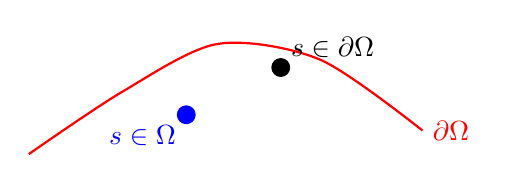
\begin{tikzpicture}[>=stealth, thick]

% Boundary curve
\draw[red, thick, smooth] plot coordinates {
  (0,0.3) (1.2,1.1) (2.4,1.7) (3.7,1.5) (5,0.6)
} node[right] {$\partial\Omega$};

% Points inside
\filldraw[blue] (2,0.8) circle (3pt) node[below left] {$s\in\Omega$};
\filldraw[black] (3.2,1.4) circle (3pt) node[above right] {$s\in\partial\Omega$};

\end{tikzpicture}
\caption{The admissibility boundary \(\partial\Omega\).}
\label{fig:boundary}
\end{figure}

% -------------------------------------------------
% Figure 5 — Cycle Structure Cₙ
% -------------------------------------------------

\begin{figure}[h!]
\centering
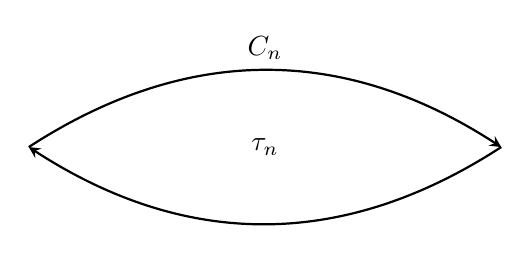
\begin{tikzpicture}[>=stealth, thick]

\draw[->] (0,0) .. controls (2,1.3) and (4,1.3) .. (6,0)
           node[midway, above] {$C_n$};
\draw[->] (6,0) .. controls (4,-1.3) and (2,-1.3) .. (0,0);

\node at (3,0) {$\tau_n$};

\end{tikzpicture}
\caption{A generic cycle \(C_n\) with period \(\tau_n\).}
\label{fig:cycle}
\end{figure}

% -------------------------------------------------
% Summary
% -------------------------------------------------

\section*{Summary}

This appendix provides TikZ-based diagrams for:

\begin{itemize}
  \item universal continuum architecture,
  \item transition operator \(\Psi_{x\to x+1}\),
  \item hierarchical structure \(K_0\)–\(K_{12}\),
  \item admissibility boundary \(\partial\Omega\),
  \item cycle structure \(C_n\).
\end{itemize}

They form the visual backbone of the Continuum Framework and are fully
synchronised with Core v2.5.



\end{document}
